
%%%%%%%%%%%%%%%%%%%%%%%%%%%%%%%%%%%%
%%%%%%%%%%%%
%
% $Autor: Wings $
% $Datum: 2019-03-05 08:03:15Z $
% $Pfad: LoRaWan.tex $
% $Version: 4250 $
% !TeX spellcheck = en_GB/de_DE
% !TeX encoding = utf8
% !TeX root = filename 
% !TeX TXS-program:bibliography = txs:///biber
%
%%%%%%%%%%%%


\chapter{LoRaWAN}
	Dieses Kapitel beschreibt die \ac{lorawan}-Architektur, die verwendeten Identifikatoren und Schlüssel, die Struktur der Protokoll-Frames sowie die Aktivierungsverfahren \acs{abp} und \acs{otaa}. Es behandelt die Eigenschaften der europäischen Frequenzbänder, Datenraten und Duty-Cycle-Vorgaben sowie die Energieaspekte der Endgeräte. Abschlie{\ss}end werden die \acs{lorawan}-Geräteklassen A, B und C sowie die Unterscheidung zwischen bestätigten und unbestätigten Nachrichten dargestellt.
	
\section{Einführung}
	LoRaWAN ermöglicht den Betrieb vieler Geräte über gro{\ss}e Distanzen hinweg \cite{Jabbar:2024a}. Das Protokoll baut auf dem physischen Layer \ac{lora} auf, dessen Modulation zur Übertragung der Datenpakete von den Endgeräten an die Empfänger verwendet wird. Die empfangenen Nachrichten werden anschlie{\ss}end über ein \ac{wan} an den entsprechenden Server bzw. die Zielanwendung weitergeleitet. LoRaWAN gewährleistet dabei die Sicherheit der übertragenen Daten und definiert zugleich die Architektur des gesamten Systems \cite{Montagny:2022}.
	
	% Picture Semtech:2024
	LoRaWAN findet in zahlreichen Bereichen Anwendung, vor allem in gro{\ss}flächig verteilten Infrastrukturen. Typische Einsatzgebiete sind die Landwirtschaft, die Luftqualitätsüberwachung, das Energiemanagement, das Flotten-Tracking, die Haussicherheit, das Parkraummanagement, die Präzisionslandwirtschaft und die intelligente Beleuchtung \cite{Seneviratne:2019, Garcia:2025, Jabbar:2024a, Jabbar:2024b, Pasetti:2020, ETSI:2018}.
	
	\begin{figure}[H]
		\centering
		\begin{tikzpicture}
			\LoRaWANTechnologyStack
		\end{tikzpicture}
		\caption{LoRaWAN-Technologiestack \cite{Semtech:2024}}
	\end{figure}

\section{Vorschriften und Normen}
	LoRaWAN basiert auf den Spezifikationen der \textit{LoRa Alliance}, insbesondere auf dem Dokument \citetitle{LoRaAlliance:2020b} \cite{LoRaAlliance:2020b} sowie der \textit{Regional Parameters Specification} \cite{LoRaAlliance:2022}.
Für den europäischen Raum (EU863–870 MHz) gelten die Vorgaben der \textit{ETSI EN 300 220}  \cite{ETSI:2018} und \textit{EN 301 489} \cite{ETSI:2019}, welche die maximal zulässige Sendeleistung, Kanalbandbreite und Duty-Cycle-Beschränkungen definieren.

\section{Netzwerkarchitektur}
	\ac{lorawan} verwendet eine sogenannte Star-of-Starts Topologie. In dieser Architektur kommunizieren die Endgeräte nicht direkt miteinander, sondern ausschlie{\ss}lich über Gateways, die als vermittler zwischen den Endgeräten und dem zentralen Netzwerkserver fungieren. Die Gateways leiten die von den Endgeräten gesendeten \ac{lora}-Pakete über eine IP-basiertes Backhaul-Netz (Ethernet, Mobilfunk, WLAN) an den Netzwerkserver weiter \cite{Semtech:2024}. Unter Backhaul versteht man in diesem Zusammenhang die kabelgebundene oder drahtlose Verbindung, über die Gateways ihre empfangenen LoRa-Pakete an den zentralen Netzwerkserver übertragen. Der Netzwerkserver übernimmt die Entschlüsselung, Duplikaterkennung und Weiterleitung der Daten an den Applikationsserver, wo die Informationen shclie{\ss}lich verarbeitet und ausgewertet werden.
	
	\begin{figure}[H]
		\centering
		\begin{tikzpicture}[scale=0.59, every node/.style={transform shape}]
			\LoRaWANinfrastructureLabel
		\end{tikzpicture}
		\caption{\ac{lorawan}-Topologie}
		\label{fig:LoRaInfrastructure}
	\end{figure}

\subsection{Endgerät}
	Ein Endgerät ist typischerweise ein Sensor oder Aktuator, der drahtlos mit dem LoRaWAN-Netzwerk verbunden ist \cite{Semtech:2024}. Es verwendet die LoRa-Modulation, um Datenpakete an die Gateways zu übertragen. Die Kommunikation erfolgt dabei mit allen Gateways, die sich in Reichweite befinden und demselben Netzwerk zugeordnet sind \cite{Montagny:2022}. Diese Geräte sind meist batteriebetriebene Einheiten, die über gro{\ss}e Flächen hinweg verteilt werden \cite{Seneviratne:2019}.


\subsection{Gateway}
	Ein Gateway empfängt die von Endgeräten innerhalb seiner Reichweite gesendeten Nachrichten und leitet diese über das IP-Backhaul (z. B. WLAN, Ethernet oder Mobilfunk) an den \ac{lns} weiter. Zwischen den Endgeräten und den Gateways besteht keine feste Zuordnung: Ein Sensor kann seine Nachricht gleichzeitig an mehrere Gateways senden, die sich in Reichweite befinden (siehe Abbildung~\ref{fig:LoRaInfrastructure}). Dieses Prinzip erhöht die Wahrscheinlichkeit eines erfolgreichen Empfangs und reduziert die Paketverlustrate, da mindestens eines der Gateways die Übertragung korrekt empfangen kann \cite{Semtech:2024}.  
	Gateways hören gleichzeitig auf allen Kanälen und Spreading Factors \cite{Montagny:2022}.
	\ac{lorawan}-Gateways arbeiten auf der physischen LoRa-Schicht. Sie empfangen die von den Endgeräten gesendeten Pakete, prüfen deren Integrität mittels einer \ac{crc}-Kontrolle und verwerfen fehlerhafte Übertragungen. Gültige Pakete werden anschlie{\ss}end zusammen mit Metadaten wie Empfangszeitstempel, RSSI und SNR an den \ac{lns} weitergeleitet. Falls Downlink-Nachrichten geplant sind, führt das Gateway die Übertragung aus, ohne den Payload zu interpretieren \cite{Semtech:2024}.
	
\subsection{Netzwerkserver}
	Der Netzwerkserver verwaltet das gesamte \ac{lorawan}-Netzwerk. Er verarbeitet die von den Gateways empfangenen, verschlüsselten Nachrichten, entfernt doppelte Pakete und gewährleistet eine sichere Übertragung durch die Verwendung von AES-128-Verschlüsselung. Dies gilt sowohl für Uplink-Nachrichten (vom Endgerät zum \ac{lns}) als auch für Downlink-Nachrichten (vom \ac{lns} zum Endgerät). Der \ac{lns} stellt sicher, dass alle Geräte im Netzwerk authentifiziert sind und die Integrität jeder Nachricht gewahrt bleibt. Dabei hat der Netzwerkserver keinen Zugriff auf den eigentlichen Anwendungsinhalt der Daten. Zudem ist der Netzwerkserver für die Anpassung des Spreading Factors und der Datenrate, das Scheduling von Downlink-Nachrichten sowie die Weiterleitung der Nachrichten an die Anwendungsserver verantwortlich \cite{Semtech:2024, Montagny:2022}.

\subsection{Anwendung}
	Die Anwendung ist für die Verarbeitung, Verwaltung und Interpretation der empfangenen Daten verantwortlich. Zudem generiert sie die Downlink-Nachrichten für die Endgeräte \cite{Semtech:2024}.

\subsection{Join Server}
	Join Server ist eine zentrale Komponente des LoRaWAN-Netzwerks die den \ac{otaa} verwaltet. Er ist für die Authentifizirung neuer Endgeräte und die Erzeugung von Sitzungscglüsseln verantwortklich \cite{Semtech:2024} \cite{LoRaAlliance:2020c}. 

% UPLINK, DOWNLINK PICTURE

\section{Frame-Struktur und Payload}
	LoRaWAN verwendet die physikalische Modulation \textbf{LoRa}, um Pakete zwischen Endgerät und Gateway zu übertragen. Dabei definiert LoRa die Struktur eines \textbf{Frames}, die wie folgt aufgebaut ist:

\begin{figure}[H]
	\centering
	\begin{tikzpicture}
		\loraframe
	\end{tikzpicture}
	\caption{Aufbau eines LoRa-Frames \cite{Semtech:2015b}}
\end{figure}

	Diese Struktur wird als \textbf{physikalische Schicht (PHY Layer)} bezeichnet. Allerdings bezieht sich dieser Aufbau ausschlie{\ss}lich auf die physikalischen Eigenschaften der Kommunikation. Das \ac{lorawan}-Protokoll ergänzt diese Schicht um zusätzliche Funktionen wie Endgeräte-Authentifizierung, Datenverschlüsselung und Bestätigung von Nachrichten. All diese Eigenschaften werden auf der darüberliegenden \textbf{MAC-Schicht} hinzugefügt und sind in der \PYTHON{MACPayload} enthalten.

	 

	\begin{figure}[H]
		\centering
		\begin{tikzpicture}
			\lorawanframes
		\end{tikzpicture}
		\caption{Aufbau der \acs{lorawan}-Frames (\cite{LoRaAlliance:2020b, Montagny:2022})}
		\label{fig:lorawan-frames}
	\end{figure}
	
	% messages tikz
\subsection{PHY Payload (\PYTHON{PHYPayload})}
	Der \PYTHON{PHYPayload} besteht aus Mac Header (\PYTHON{MHDR}), \hyperref[lorawan:macPayload]{Mac Payload (\PYTHON{MACPayload})} und \hyperref[lorawan:mic]{\acl{mic} (\PYTHON{MIC})} 
	
	\begin{figure}[H]
		\centering
		\begin{tikzpicture}
			\phyPayload
		\end{tikzpicture}
		\caption{Darstellung des \PYTHON{PHYPayload} \cite{LoRaAlliance:2020b}}
	\end{figure}
	
	
	
\subsubsection{Mac Header (\PYTHON{MHDR})}
	\begin{figure}[H]
		\centering
		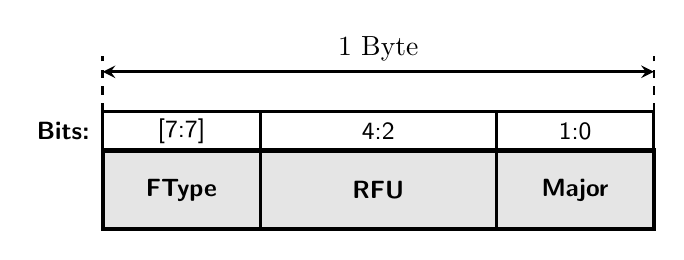
\begin{tikzpicture}
			\tikzset{
				defaulttext/.style={
					font=\sffamily\small,
				},
				smallText/.style={
					font=\sffamily\footnotesize,
				},
				defaultDashed/.style={dashed,line width=0.03cm},
				lineDef/.style={line width={1.5pt}},
				lineScaled/.style={line width={1pt}},
				arrowStyle/.style={lineScaled, >=stealth},
			}
			\draw[lineDef, fill=gray!20] (0,0) rectangle (7, 1.0);
			
			\foreach \x in {0, 2, 5, 7} {
				\draw[lineScaled] (\x, 0) -- (\x, 1.5);
			}
			
			\foreach \x in {0, 7} {
				\draw[defaultDashed] (\x, 1.5) -- (\x, 2.2);
			}
			
			\draw[lineScaled] (0,1.5) -- (7, 1.5);
			
			\node[defaulttext] at (1, 0.5) {\textbf{FType}};
			\node[defaulttext] at (1, 1.25) {\text{[7:7]}};
			\node[defaulttext] at (3.5, 0.5) {\textbf{RFU}};
			\node[defaulttext] at (3.5, 1.25) {\text{4:2}};
			\node[defaulttext] at (6, 0.5) {\textbf{Major}};
			\node[defaulttext] at (6, 1.25) {\text{1:0}};
			\node[defaulttext] at (-0.5, 1.25) {\textbf{Bits:}};
			%size
			\draw[arrowStyle, <->] (0, 2) -- node[midway, above] {1 Byte} (7,2);
			
		\end{tikzpicture}
		\caption{Liste der Major-Versionen \cite{LoRaAlliance:2020b}}
	\end{figure}
	

	Der \ac{mac}-Header gibt den Typ des Frames sowie die Major-Version des Frame-Formats an \cite[15]{LoRaAlliance:2020b}. \ac{lorawan} unterscheidet acht verschiedene Typen von \ac{mac}-Frames:
	\begin{table}[H]
		\centering
		\begin{tabular}{|p{2cm}|p{3cm}|}
			\hline
			\textbf{FType} & \textbf{Description} \\ \hline
			000 & Join-Request \\ \hline
			001 & Join-Accept \\ \hline
			010 & Unconfirmed Data Uplink \\ \hline
			011 & Unconfirmed Data Downlink \\ \hline
			100 & Confirmed Data Uplink \\ \hline
			101 & Confirmed Data Downlink \\ \hline
			110 & RFU \\ \hline
			111 & Proprietary \\ \hline
		\end{tabular}
		\caption{FType-Werte und ihre Bedeutung \cite{LoRaAlliance:2020b}}
	\end{table}
	

	Das \textbf{Major-Feld} im \PYTHON{MHDR} gibt die Hauptversion des LoRaWAN-Protokolls an, nach der die übertragenen Frames aufgebaut sind. Der Wert 00 steht für das Format LoRaWAN R1, das in allen aktuellen Netzwerken verwendet wird. Andere Werte (01 – 11) sind als Reserved for Future Use (RFU) vorgesehen und dienen der zukünftigen Erweiterung des Standards. Das Major-Feld stellt somit sicher, dass Endgeräte und Netzwerkserver denselben Frame-Aufbau verwenden und korrekt miteinander kommunizieren können \cite{LoRaAlliance:2020b}.
	\begin{table}[H]
		\centering
		\begin{tabular}{|c|l|}
			\hline
			\textbf{Major} & \textbf{Description} \\ \hline
			00 & LoRaWAN R1 \\ \hline
			01..11 & RFU \\ \hline
		\end{tabular}
		\caption{Major list \cite{LoRaAlliance:2020b}}
	\end{table}

\subsubsection{Message Integrity Code (\PYTHON{MIC}) \label{lorawan:mic}}  
	Der \PYTHON{MIC} funktioniert wie eine digitale Unterschrift. Zur Berechnung dieses Codes wird der \textit{Cipher-based Message Authentication Code} (CMAC) auf Basis von \textbf{AES-128} über alle Felder des zu übertragenden Pakets (\PYTHON{PHYPayload}) gebildet. Der \PYTHON{MIC} hat eine Länge von 4~Byte und besteht aus den ersten vier Byte des berechneten CMAC-Werts. Dabei muss sichergestellt werden, dass der \hyperref[lorawan:frmpayload]{\PYTHON{FRMPayload}} vor der Berechnung des \PYTHON{MIC} noch verschlüsselt ist \cite[24]{LoRaAlliance:2020b}.
	
	\begin{align*}
		msg &= MHDR \,|\, FHDR \,|\, FPort \,|\, FRMPayload \\
		CMAC &= aes128\_cmac(NwkSKey, B_0 \,|\, msg)	\\
		MIC &= CMAC[0..3]
	\end{align*}
	
	Der Block \( B_0 \) wird wie folgt definiert:  
	
	\[
	B_0 = 0x49 \,|\, 0x00\,0x00\,0x00\,0x00 \,|\, Dir \,|\, DevAddr \,|\, FCnt \,|\, 0x00 \,|\, len(msg)
	\]
	
	Der MIC wird auf der Empfängerseite erneut berechnet. Stimmt der berechnete Wert nicht mit dem empfangenen überein, bedeutet dies, dass die Daten manipuliert wurden und die Nachricht verworfen wird. Dieser Code wird mithilfe aller inhalte vom jeweiligen Paket berechnet und am ende eines jeweilgen Paket hinzugefügt \cite[25]{LoRaAlliance:2020b}
	
		\begin{figure}[H]
		\centering
		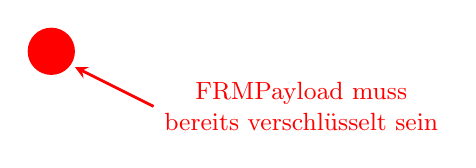
\begin{tikzpicture}
			\micEncryption
			\fill[red] (6.5, 2) circle (0.3cm);
			\lock{0.15}{0}{6.5}{1.95}
			\draw[red, arrowStyle, <-] (6.8,1.8) -- ++(1,-0.5) node[right] {\small\shortstack{\PYTHON{FRMPayload} muss \\ bereits verschlüsselt sein}};
		\end{tikzpicture}
		\caption{Schematische Darstellung der \PYTHON{MIC}-Berechnung \cite{Montagny:2022}}
	\end{figure}
	
		
\subsection{MAC Payload (\PYTHON{MACPayload}) \label{lorawan:macPayload}}
	Die \PYTHON{MACPayload} besteht aus dem \hyperref[lorawan:frameHeader]{Frame Header (\PYTHON{FHDR})}, gefolgt vom optionalen Port-Feld (\PYTHON{FPort}) und dem optionalen Payload-Feld (\PYTHON{FRMPayload}).
	\begin{figure}[H]
		\centering
		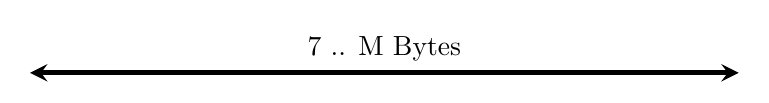
\begin{tikzpicture}
			\macPayload
			
			\draw[line width=0.06cm, <->, >=stealth](3, -2.7) -- node[midway, above]{7 .. M Bytes} (12, -2.7);
		\end{tikzpicture}
		\caption{Darstellung des \PYTHON{MACPayload} \cite{LoRaAlliance:2020b}}
	\end{figure}
	
	Der maximale Länge der \PYTHON{MACPayload} hängt von der verwendeten Region ab.  
	\citetitle[Kap.~2.4.6]{LoRaAlliance:2022} nennt folgende Werte:
	
	\begin{table}[H]
		\centering
		\begin{tabular}{|c|c|c|}
			\hline
			\textbf{Data Rate} & \textbf{M} & \textbf{N} \\ \hline
			0 & 59 & 51 \\ \hline
			1 & 59 & 51 \\ \hline
			2 & 59 & 51 \\ \hline
			3 & 123 & 115 \\ \hline
			4 & 230 & 222 \\ \hline
			5 & 230 & 222 \\ \hline
			6 & 230 & 222 \\ \hline
			7 & 230 & 222 \\ \hline
			8 & 58 & 50 \\ \hline
			9 & 123 & 115 \\ \hline
			10 & 58 & 50 \\ \hline
			11 & 123 & 115 \\ \hline
			12--15 & \textit{Nicht definiert} & \textit{Nicht definiert} \\ \hline
		\end{tabular}
		\caption{EU863–870: maximale \PYTHON{MACPayload}-Grö{\ss}e in Bytes \cite{LoRaAlliance:2022}}
		\label{tab:lorawan-payload-m}
	\end{table}
	
	Wenn das Feld \PYTHON{FOpts} (in \PYTHON{FHDR}) keine Inhalte enthält, können die Applikationsdaten (\PYTHON{FRMPayload}) die Grö{\ss}e \textbf{N} erreichen. Der Wert von \textbf{N} kann jedoch kleiner sein, wenn das Feld \PYTHON{FOpts} nicht leer ist \cite[Kap. 2.4.6]{LoRaAlliance:2022}.  
	Die gesendete Payload darf die maximale Grö{\ss}e nicht überschreiten, da die Nachricht sonst vom Server verworfen wird \cite[15]{LoRaAlliance:2020b}.

	
	
\subsubsection{Port Field (\PYTHON{FPort})}
	Das \PYTHON{FPort}-Feld wird verwendet, um den Typ der übertragenen Daten zu kennzeichnen. Ein Wert von 0 bedeutet, dass die Nachricht ausschlie{\ss}lich \ac{mac}-Befehle enthält. Werte zwischen 1 und 223 sind für applikationsspezifische Daten vorgesehen. Die Werte 224 - 255 sind für die Nutzung und Allokation durch die \ac{lorawan}~Alliance reserviert \cite[23]{LoRaAlliance:2020b}.

\subsubsection{Frame-Payload (\PYTHON{FRMPayload}) \label{lorawan:frmpayload}}
	Das Feld \PYTHON{FRMPayload} ist der Hauptträger der Nutzlast im \ac{lorawan}-Frame. Es enthält die eigentlichen Applikationsdaten, die zwischen Endgerät und Server ausgetauscht werden. Der Inhalt und die Interpretation dieses Feldes hängen vom Wert des \PYTHON{FPort}-Feldes ab. Die darin enthaltenen Daten werden stets verschlüsselt.

	Wenn \PYTHON{FPort} gleich 0 ist, werden in \PYTHON{FRMPayload} ausschlie{\ss}lich \hyperref[lorawan:macCommands]{\ac{mac}-Befehle} übertragen, die zur Verwaltung der Netzkommunikation dienen. Sie werden mithilfe des \hyperref[lorawan:NwkSKey]{\PYTHON{NwkSKey}} verschlüsselt.  
	
	\begin{figure}[H]
		\centering
		\begin{tikzpicture}
			\frmPayloadEncryptionMAC
		\end{tikzpicture}
		\caption{Schematische Darstellung der \PYTHON{FRMPayload}-Verschlüsselung \cite{Montagny:2022}}
	\end{figure}
	
	Wenn \PYTHON{FPort} die Werte zwischen 1 und 225 enthält das Feld applikationsspezifische Daten, die direkt an die jeweilige Anwendung weitergeleitet werden. Diese Applikationsdaten im \PYTHON{FRMPayload}-Feld werden mit dem \hyperref[lorawan:AppSKey]{\PYTHON{AppSKey}} verschlüsselt, um die Vertraulichkeit und Authentizität der übertragenen Informationen zu gewährleisten. Dadurch wird verhindert, dass Dritte den Inhalt der Nachricht lesen oder verändern können.
	
		\begin{figure}[H]
			\centering
			\begin{tikzpicture}
				\frmPayloadEncryptionAPP
			\end{tikzpicture}
			\caption{Schematische Darstellung der \PYTHON{FRMPayload}-Verschlüsselung \cite{Montagny:2022}}
	\end{figure}

	Es ist zu beachten, dass dieses Feld verschlüsselt werden muss, bevor der \hyperref[lorawan:mic]{\PYTHON{MIC}} berechnet wird \cite{LoRaAlliance:2020b, Montagny:2022}.


% tikz verschlüsseln
\subsection{Frame-Header (\PYTHON{FHDR}) \label{lorawan:frameHeader}}
	Die \PYTHON{FHDR} besteht aus der Endgeräteadresse \hyperref[lorawan:deviceAddr]{\PYTHON{DevAddr}}, dem Frame-Control-Byte \PYTHON{FCtrl}, einem 2 Bytes langen Frame Counter (\PYTHON{FCnt}) sowie bis zu 15 Bytes an Frame Options (\PYTHON{FOpts}).
	 
	\begin{figure}[H]
		\centering
		\begin{tikzpicture}
			\fhdrHeader
		\end{tikzpicture}
		\caption{Darstellung der \PYTHON{FHDR}-Felder und ihrer Länge in Bytes \cite{LoRaAlliance:2020b}}
	\end{figure}
	

\subsubsection{\PYTHON{FCtrl} für downlink Frames}
	\begin{figure}[H]
		\centering
		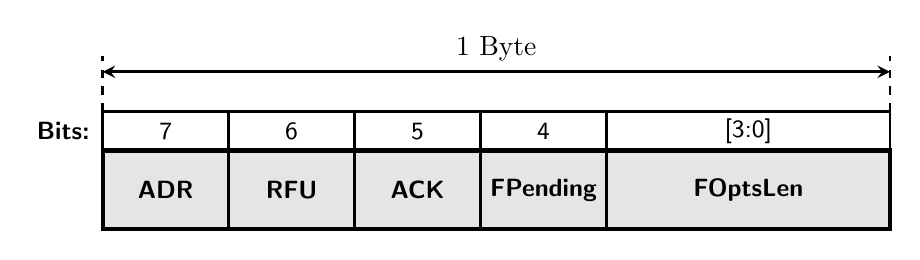
\begin{tikzpicture}
			\tikzset{
				defaulttext/.style={
					font=\sffamily\small,
				},
				smallText/.style={
					font=\sffamily\footnotesize,
				},
				defaultDashed/.style={dashed,line width=0.03cm},
				lineDef/.style={line width={1.5pt}},
				lineScaled/.style={line width={1pt}},
				arrowStyle/.style={lineScaled, >=stealth},
			}
			\draw[lineDef, fill=gray!20] (0,0) rectangle (10, 1.0);
			
			\foreach \x in {0, 1.6, 3.2, 4.8, 6.4 ,10} {
				\draw[lineScaled] (\x, 0) -- (\x, 1.5);
			}
			
			\foreach \x in {0, 10} {
				\draw[defaultDashed] (\x, 1.5) -- (\x, 2.2);
			}
			
			\draw[lineScaled] (0,1.5) -- (10, 1.5);
			
			\node[defaulttext] at (0.8, 0.5) {\textbf{ADR}};
			\node[defaulttext] at (0.8, 1.25) {\text{7}};
			\node[defaulttext] at (2.4, 0.5) {\textbf{RFU}};
			\node[defaulttext] at (2.4, 1.25) {\text{6}};
			\node[defaulttext] at (4, 0.5) {\textbf{ACK}};
			\node[defaulttext] at (4, 1.25) {\text{5}};
			\node[defaulttext] at (5.6, 0.5) {\textbf{FPending}};
			\node[defaulttext] at (5.6, 1.25) {\text{4}};
			\node[defaulttext] at (8.2, 0.5) {\textbf{FOptsLen}};
			\node[defaulttext] at (8.2, 1.25) {\text{[3:0]}};
			\node[defaulttext] at (-0.5, 1.25) {\textbf{Bits:}};
			
			%size
			\draw[arrowStyle, <->] (0, 2) -- node[midway, above] {1 Byte} (10,2);
			
		\end{tikzpicture}
		\caption{FCtrl Downlink Frame Format}
	\end{figure}
	
	\begin{itemize}
		\item \PYTHON{ADR} wird verwendet, um die adaptive Datenrate \PYTHON{ADR} zu aktivieren oder zu deaktivieren (siehe~\ref{lorawan:adr}).
		\item \PYTHON{RFU} ist für zukünftige Verwendung reserviert (Reserved for Future Use).
		\item \PYTHON{ACK} wird verwendet, um eine erfolgreiche Bestätigung (Acknowledgment) eines empfangenen Uplink-Frames anzuzeigen.
		\item \PYTHON{FPending} zeigt an, dass auf dem Netzwerkserver weitere Downlink-Nachrichten für das Endgerät zur Verfügung stehen.
		\item \PYTHON{FOptsLen} gibt die aktuelle Länge des Frame-Options-Feldes \PYTHON{FOpts} an \cite{LoRaAlliance:2020b}.
	\end{itemize}
	
	
\subsubsection{\PYTHON{FCtrl} für uplink Frames}
	\begin{figure}[H]
		\centering
		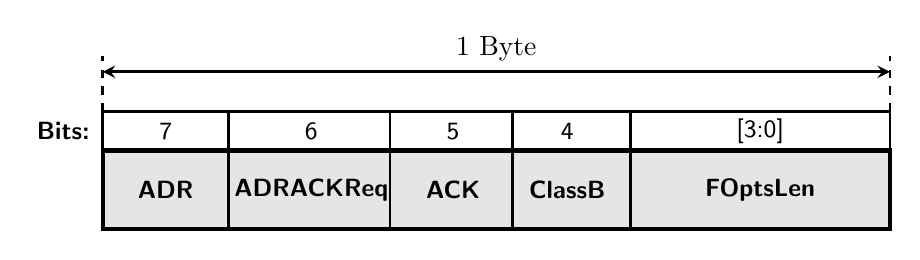
\begin{tikzpicture}
			\tikzset{
				defaulttext/.style={
					font=\sffamily\small,
				},
				smallText/.style={
					font=\sffamily\footnotesize,
				},
				defaultDashed/.style={dashed,line width=0.03cm},
				lineDef/.style={line width={1.5pt}},
				lineScaled/.style={line width={1pt}},
				arrowStyle/.style={lineScaled, >=stealth},
			}
			\draw[lineDef, fill=gray!20] (0,0) rectangle (10, 1.0);
			
			\foreach \x in {0, 1.6, 3.65, 5.2, 6.7 ,10} {
				\draw[lineScaled] (\x, 0) -- (\x, 1.5);
			}
			
			\foreach \x in {0, 10} {
				\draw[defaultDashed] (\x, 1.5) -- (\x, 2.2);
			}
			
			\draw[lineScaled] (0,1.5) -- (10, 1.5);
			
			\node[defaulttext] at (0.8, 0.5) {\textbf{ADR}};
			\node[defaulttext] at (0.8, 1.25) {\text{7}};
			\node[defaulttext] at (2.65, 0.5) {\textbf{ADRACKReq}};
			\node[defaulttext] at (2.65, 1.25) {\text{6}};
			\node[defaulttext] at (4.45, 0.5) {\textbf{ACK}};
			\node[defaulttext] at (4.45, 1.25) {\text{5}};
			\node[defaulttext] at (5.9, 0.5) {\textbf{ClassB}};
			\node[defaulttext] at (5.9, 1.25) {\text{4}};
			\node[defaulttext] at (8.35, 0.5) {\textbf{FOptsLen}};
			\node[defaulttext] at (8.35, 1.25) {\text{[3:0]}};
			\node[defaulttext] at (-0.5, 1.25) {\textbf{Bits:}};
			
			%size
			\draw[arrowStyle, <->] (0, 2) -- node[midway, above] {1 Byte} (10,2);
			
		\end{tikzpicture}
		\caption{FCtrl Uplink Frame Format}
	\end{figure}
	
	\begin{itemize}
		\item \PYTHON{ADR} und \PYTHON{ADRACKReq} werden bei der Verwendung der adaptiven Datenrate \PYTHON{ADR} eingesetzt (siehe~\ref{lorawan:adr}).
		\item \PYTHON{ACK} wird verwendet, wenn eine Bestätigung (Acknowledgment) erforderlich ist.
		\item \PYTHON{ClassB} wird nur bei einem Uplink auf 1 gesetzt, wenn das Gerät im Klassenmodus~B arbeitet und bereit ist, Beacons zu empfangen (siehe \ref{lorawan:deviceClassB}).
		\item \PYTHON{FOptsLen} gibt die aktuelle Länge des Frame-Options-Feldes \PYTHON{FOpts} in Bytes an \cite{LoRaAlliance:2020b}.
	\end{itemize}
	
	\subsubsection{Frame Options (\PYTHON{FOpts})}
	Das Feld \PYTHON{FOpts} transportiert \ac{mac}-Befehle mit einer maximalen Länge von 15~Bytes.  
	Diese Befehle werden direkt im Frame Header (\PYTHON{FHDR}) übertragen. Die tatsächliche Länge des Feldes wird durch das Feld \PYTHON{FOptsLen} im \PYTHON{FCtrl}-Byte angegeben.  
	
	\noindent
	\textbf{Hinweis:} \ac{mac}-Befehle können entweder im Feld \PYTHON{FOpts} oder im Feld \PYTHON{FRMPayload} übertragen werden, jedoch niemals gleichzeitig in beiden (siehe~\autoref{lorawan:frmpayload}). Befinden sich die Befehle im Feld \PYTHON{FOpts}, muss das Feld \PYTHON{FPort} ungleich 0 sein.  Werden die Befehle dagegen im Feld \PYTHON{FRMPayload} übertragen, muss \PYTHON{FPort} den Wert 0 haben.  
	
	Gemä{\ss} der \citetitle{LoRaAlliance:2020b} muss eine Nachricht verworfen werden, wenn \ac{mac}-Befehle gleichzeitig in beiden Feldern vorhanden sind \cite{LoRaAlliance:2020b}.
	

\section{Verschlüsselung und Sicherheit}
	In \ac{lorawan} werden mehrere eindeutige Identifikatoren und kryptografische Schlüssel verwendet, um jedes Endgerät eindeutig zuzuordnen und die Kommunikation abzusichern. Dabei spielen sowohl statische, herstellerseitig vergebene Nummern als auch dynamisch erzeugte Netzwerkadressen eine Rolle.
	
	\subsection{Geräte- und Anwendungsidentifikatoren}
	
	\subsubsection{\acl{deveui} \PYTHON{DevEUI}}
	Ein weltweit eindeutiger, 64~Bit langer Identifikator, der vom Gerätehersteller vergeben und im Modul dauerhaft gespeichert wird. Er dient zur eindeutigen Identifizierung des Endgeräts bei der Aktivierung über \ac{otaa} \cite[44]{LoRaAlliance:2022} \cite{Montagny:2022}.
	
	\subsubsection{\acl{joineui} \PYTHON{JoinEUI}}
	Ebenfalls 64~Bit lang, identifiziert die Anwendung bzw. den Join-Server, an den sich das Gerät bei der Aktivierung wendet. Dieser Identifikator muss vor dem Join-Prozess auf dem Endgerät gespeichert sein \cite[44]{LoRaAlliance:2022}.
	
	
	\subsubsection{\acl{devaddr} \PYTHON{DevAddr} \label{lorawan:deviceAddr}}
	Eine 32~Bit lange Geräteadresse, die das Endgerät innerhalb des Netzwerks identifiziert. Sie wird vom \ac{lns} bei jeder neuen Sitzung (\ac{otaa}) dynamisch vergeben \cite[42]{LoRaAlliance:2022}
	
	
	\subsection{Kryptografische Schlüssel}
	Durch die Trennung der Schlüsselbereiche zwischen Endgerät, Netzwerk- und Anwendungsserver wird in \ac{lorawan} eine echte End-to-End-Sicherheit erreicht. Der Netzwerkserver kann die übertragenen Nutzdaten weder entschlüsseln noch verändern, was einen hohen Schutz der Benutzerdaten gewährleistet \cite[43]{Montagny:2022}.
	
	\subsubsection{\acl{appkey} \PYTHON{AppKey}}
	Der \PYTHON{AppKey} ist ein eindeutiger, 128~Bit langer Hauptschlüssel, der jedem Endgerät individuell zugeordnet wird. Er wird sowohl auf dem Endgerät als auch auf dem Join-Server gespeichert und niemals über das Netzwerk übertragen. Der Schlüssel wird verwendet, um bei Verbindungsaufbauten über \ac{otaa} neue Sitzungsschlüssel (\PYTHON{AppSKey} und \PYTHON{NwkSKey}) für das jeweilige Endgerät zu generieren \cite[44]{LoRaAlliance:2020b}.
	
	\subsubsection{\acl{nwkskey} \PYTHON{NwkSKey} \label{lorawan:NwkSKey}}
	Der \PYTHON{NwkSKey} (128~Bit) ist ein \textbf{Sitzungsschlüssel} und wird verwendet, um die Integrität der Endgeräte sicherzustellen und Manipulationen zu verhindern. Dieser Schlüssel wird für die Berechnung eines sogenannten \hyperref[lorawan:mic]{\textit{Message Integrity Code} (MIC)} verwendet, der an jedes übertragene Paket angehängt wird \cite[43]{LoRaAlliance:2020b} \cite[43]{Montagny:2022}.  
	
	\subsubsection{\acl{appskey} \PYTHON{AppSKey} \label{lorawan:AppSKey}}
	Der \PYTHON{AppSKey} (128~Bit) \textbf{Sitzungsschlüssel} und dient zur Verschlüsselung der Benutzerdaten (\PYTHON{FRMPayload}), die über \ac{lorawan} übertragen werden.  Die Verschlüsselung findet im Endgerät für Uplink-Nachrichten bzw. in der Anwendung für Downlink-Nachrichten statt. Die Entschlüsselung erfolgt jeweils auf der gegenüberliegenden Seite – also in der Anwendung für Uplink und im Endgerät für Downlink.  Gateway und Netzwerkserver haben somit keinen Zugriff auf die eigentlichen Inhalte der Nachricht \cite[43]{LoRaAlliance:2020b} \cite[43]{Montagny:2022}.  Diese Verschlüsselung basiert auf dem \textbf{AES-128}-Algorithmus mit einer Schlüssellänge von 128~Bit \cite[24]{LoRaAlliance:2020b}.
	
	
	\begin{figure}[H]
		\centering
		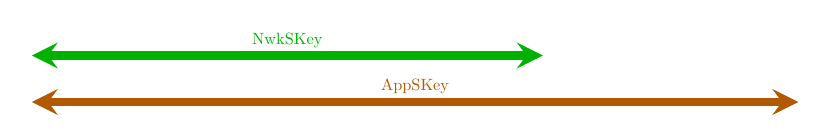
\begin{tikzpicture}[scale=0.59, every node/.style={transform shape}]
			\tikzset{
				lineScaled/.style={line width={3pt}},
				arrowStyle/.style={lineScaled, >=stealth},
			}
			\LoRaWANinfrastructure
			\draw[arrowStyle, <->, green!70!black] (3, 0) -- node[midway, above] {\PYTHON{NwkSKey}} (14, 0);
			\draw[arrowStyle, <->, orange!70!black] (3, -1) -- node[midway, above] {\PYTHON{AppSKey}} (19.5, -1);
		\end{tikzpicture}
		\caption{Darstellung des Zuständigkeitsbereichs der Sitzungsschlüssel \cite{Montagny:2022}}
	\end{figure}
	
\section{Aktivierung des Endgeräts (OTAA und ABP)}  
	In \ac{lorawan} können Endgeräte auf zwei Arten aktiviert werden:  
	\begin{itemize}
		\item \textbf{\acf{abp}}
		\item \textbf{\acf{otaa}} 
	\end{itemize}
	Für die Authentifizierung werden jeweils \ac{appskey}, \ac{nwkskey} und \ac{devaddr} verwendet.

\subsection{\acf{abp}}
	Die Sitzungsschlüssel (\PYTHON{AppSKey} und \PYTHON{NwkSKey}) sowie die \PYTHON{DevAddr} sind dauerhaft im Gerät und auf dem Netzwerkserver gespeichert und werden nicht dynamisch erzeugt. Diese Schlüsseln werden bei jeder Sitzung verwendet. Allerdings besitzt jedes Endgerät individuelle Sitzungsschlüssel, sodass im Falle einer Kompromittierung nicht automatisch alle Geräte betroffen sind \cite[48]{Semtech:2024}. Diese Methode ist zwar einfach in der Handhabung, bietet jedoch ein geringeres Sicherheitsniveau, da die Schlüssel nicht regelmä{\ss}ig erneuert werden \cite{Montagny:2022}.

\subsection{\acf{otaa}}
	Bei der \ac{otaa} werden die Sitzungsschlüssel dynamisch generiert, wodurch jede Verbindung eine eigene, eindeutige Sicherheitssitzung erhält. Dies erhöht die Datensicherheit erheblich, da bei jeder erneuten Aktivierung neue Schlüsselpaare (\PYTHON{NwkSKey} und \PYTHON{AppSKey}) abgeleitet werden. Die Schlüssel werden auf Basis des Hauptschlüssels (\PYTHON{AppKey}) gebildet, der sowohl auf dem Endgerät als auch auf dem Join Server hinterlegt ist. Auf diese Weise wird gewährleistet, dass die übertragene Kommunikation zwischen Endgerät und Netzwerk stets kryptografisch geschützt und voneinander isoliert bleibt \cite{LoRaAlliance:2020b, Semtech:2024, Montagny:2022}

\subsection{Weitere Parameter bei Verwendung von \ac{otaa}}
	\begin{itemize}
		\item \textbf{\acl{devnonce}} \PYTHON{DevNonce} - Die \PYTHON{DevNonce} ist ein Zähler, der beim Start des Systems mit dem Wert~0 beginnt und sich bei jeder \textit{Join Request}-Nachricht um~1 erhöht. Wird das Endgerät regelmä{\ss}ig ausgeschaltet, muss die \PYTHON{DevNonce} in einem nichtflüchtigen Speicher (\textit{non-volatile memory}) gesichert werden, damit der Zählerwert nach einem Neustart erhalten bleibt. Wird die \PYTHON{DevNonce} zurückgesetzt oder die \PYTHON{JoinEUI} geändert, verwirft der JoinServer alle \textit{Join Request}-Nachrichten, da er die zuletzt verwendete \PYTHON{DevNonce} jedes Geräts speichert, um Wiederholungsangriffe zu verhindern \cite[45]{LoRaAlliance:2020b}.
		\item \textbf{\acl{joinnonce}} \PYTHON{JoinNonce}- Eine Zufallszahl, die während des Join-Prozesses vom Join Server erzeugt wird. Sie wiederholt sich nie und wird verwendet, um nach der Join-Prozedur die \PYTHON{NwkSKey} und \PYTHON{AppSKey} zu generieren \cite[46]{LoRaAlliance:2020b}.
	\end{itemize}

\subsection{Join-Prozedur}
	Zu Beginn müssen dem Gerät der \PYTHON{AppKey}, die \PYTHON{JoinEUI} und die \PYTHON{DevEUI} bekannt sein. Die Join-Prozedur besteht aus zwei MAC-Paketen: \textit{Join Request} und \textit{Join Accept}.

\subsubsection{Join-Request Frame}
	Zuerst wird ein \textit{Join Request}-Frame vom Endgerät an den Join Server gesendet.
	\begin{figure}[H]
		\centering
		\begin{tikzpicture}
			\phyLayerFrame
			\JoinRequestFrame{1}{0}{4}{-1.1}
			\draw[defaultDashed] (AphyLayer) -- (Areq);
			\draw[defaultDashed] (BphyLayer) -- (Breq);
			
		\end{tikzpicture}
		\caption{Struktur des \textit{Join-Request}-Frames \cite{LoRaAlliance:2020b}}
	\end{figure}
		
 Der \textit{Join Request}-Frame wird vollständig im \PYTHON{PHYPayload} untergebracht \cite{LoRaAlliance:2020b}
		 
		 
		 
	% tikz Semtech2024
\subsubsection{Join-Accept Frame}
	Nachdem das Gerät erfolgreich authentifiziert wurde, sendet der JoinServer ein \textit{Join Accept}-Frame an das Endgerät.
		\begin{figure}[H]
			\centering
			\begin{tikzpicture}
				\phyLayerFrame
				\JoinAcceptFrame{1}{0}{1}{-1.1}
				\draw[defaultDashed] (AphyLayer) -- (Areq);
				\draw[defaultDashed] (BphyLayer) -- (Breq);
			\end{tikzpicture}
			\caption{Struktur des \textit{Join-Accept}-Frames \cite{LoRaAlliance:2020b}}
		\end{figure}
\subsubsection{Berechnung der Sitzungsschlüssel}
	Im nächsten Schritt berechnet das Endgerät auf Basis von \PYTHON{DevEUI}, \PYTHON{JoinEUI}, \PYTHON{DevNonce}, den Hauptschlüssel (\PYTHON{AppKey}) sowie den Feldern der \textit{Join Request}- und \textit{Join Accept}-Nachrichten seine Sitzungsschlüssel. Der JoinServer berechnet dieselben Schlüssel und teilt sie mit dem \ac{lns} und dem Anwendung Server, um die Kommunikation zwischen Endgerät, Netzwerk- und Anwendungsserver abzusichern.
	% tikz Semtech2024

\subsubsection{Ablauf des Join-Prozesses}
\begin{figure}[H]
	\centering
	\begin{tikzpicture}
		\OTAActivationProcedure
	\end{tikzpicture}
	\caption{Ablauf des Join-Prozesses \cite{LoRaAlliance:2020c}}
\end{figure}
\subsubsection{Netzwerkserver als Join Server}
	Ein separater Join Server ist nicht zwingend erforderlich. Verfügt man nur über eine kleine Infrastruktur oder bestehen die Endgeräte aus selbst entwickelten DIY-Lösungen ohne eigenen Join Server, kann der \ac{lns} die Funktion des Join Servers übernehmen. In diesem Fall verwaltet der \ac{lns} die \textit{Join Requests} und übernimmt die Generierung der Sitzungsschlüssel für die Endgeräte \cite{Montagny:2022}


\section{Frequenzbänder und Kanäle (EU863–870)}
In Europa nutzt LoRaWAN überwiegend das lizenzfreie ISM-Band von 863 MHz bis 870 MHz.
Typischerweise sind acht Standardkanäle mit 125 kHz Bandbreite sowie ein zusätzlicher Kanal mit 250 kHz für Datenraten zwischen SF7 und SF12 definiert.
Die zulässige äquivalente isotrope Sendeleistung (EIRP) beträgt in der Regel 14 dBm.



\section{Geräteklassen}
	\textcite{LoRaAlliance:2020b} beschreibt drei Klassen von \ac{lorawan}-Endgeräten. Diese Klassen definieren das Verhalten der Geräte hinsichtlich Energieverbrauch und Bereitschaft zum Empfang von Downlink-Nachrichten. Klasse~A ist die Hauptklasse, in der alle \ac{lorawan}-Geräte grundsätzlich arbeiten müssen. Geräte der Klassen~B und~C müssen daher ebenfalls in der Lage sein, im Modus der Klasse~A zu funktionieren.

\subsection{Klasse~A \label{lorawan:deviceClassA}}
	In dieser Klasse befindet sich das Endgerät die meiste Zeit im \textbf{Ruhezustand}, um Energie zu sparen. Nach jeder Uplink-Übertragung öffnen sich zwei Empfangsfenster: \textbf{RX1} und \textbf{RX2}. Der \ac{lns} bzw. das Gateway kann eine Downlink-Nachricht in \textit{einem} dieser Fenster senden, jedoch nicht in beiden. Wird die Präambel einer Downlink-Nachricht innerhalb eines Empfangsfensters erkannt, bleibt das Funkmodul während der gesamten Übertragungs- und Demodulationszeit aktiv. Empfängt und demoduliert das Gerät erfolgreich eine Downlink-Nachricht im \textbf{RX1}-Fenster, so wird das zweite Fenster (\textbf{RX2}) nicht mehr geöffnet \cite[13]{LoRaAlliance:2020b}, \cite[45]{Montagny:2022} \cite[22]{Semtech:2024}.

	Es ist zu beachten, dass ein Gerät der Klasse~A beide Downlink-Fenster (\textbf{RX1} und \textbf{RX2}) abwarten muss, bevor eine neue Nachricht gesendet werden kann \cite[13]{LoRaAlliance:2020b}.

	\begin{figure}[H]
		\raggedright
		\begin{tikzpicture}
			\deviceClassAnothingReceives
		\end{tikzpicture}
		\caption{Kein Downlink empfangen: Beide Empfangsfenster (RX1 und RX2) bleiben ohne Downlink \cite{Semtech:2024}}
	\end{figure}
	
	\begin{figure}[H]
		{
		\raggedright
		\begin{tikzpicture}
			\deviceClassArecRxOne
		\end{tikzpicture}
		}
		\caption{Downlink in RX1: Das Endgerät empfängt die Downlink-Übertragung im ersten Empfangsfenster \cite{Semtech:2024}}
	\end{figure}
	
	
	\begin{figure}[H]
		\raggedright
		\begin{tikzpicture}
			\deviceClassArecRxTwo
		\end{tikzpicture}
		\caption{Downlink in RX2: Das Endgerät empfängt die Downlink-Übertragung im zweiten Empfangsfenster \cite{Semtech:2024}}
	\end{figure}
	
	\begin{figure}[H]
		\centering
		\begin{tikzpicture}
			\deviceClassA
		\end{tikzpicture}
	\caption{Darstellung der Uplink- und Downlink-Fenster \cite{Semtech:2024}}
	\end{figure}

% lora class A

\subsubsection{RX1 Fenster}
	Das erste Empfangsfenster (\textbf{RX1}) öffnet sich spätestens \PYTHON{RECEIVE\_DELAY1} Sekunden nach dem Ende der Uplink-Übertragung, wobei \PYTHON{RECEIVE\_DELAY1} typischerweise im Bereich von 1~s bis 15~s liegt \cite[12]{LoRaAlliance:2020b}. Standardmä{\ss}ig nutzt das RX1-Fenster denselben Kanal wie der vorherige Uplink, 
	wobei die Datenrate eine Funktion der Uplink-Datenrate und des Parameters \PYTHON{RX1DROffset} ist \cite[35]{LoRaAlliance:2022}. Die Zuordnung zwischen Uplink- und \textbf{RX1}-Datenraten ist in Form einer Tabelle im Kapitel ,,EU863-870 Receive Windows'' des Dokuments \textcite{LoRaAlliance:2022} dargestellt.
	
\subsubsection{RX2 Fenster}
	Das zweite Empfangsfenster (\textbf{RX2}) öffnet sich spätestens \PYTHON{RECEIVE\_DELAY2} Sekunden nach der Uplink-Übertragung, wobei \PYTHON{RECEIVE\_DELAY2} typischerweise zwischen 2 s und 16 s liegt \cite[12]{LoRaAlliance:2020b}. Das RX2-Fenster verwendet eine feste Frequenz und Datenrate; die Standardparameter für die EU868-Region betragen 869{,}525 MHz / DR0 (SF12, 125 kHz) \cite[35]{LoRaAlliance:2022}.


	
\subsection{Klasse~B \label{lorawan:deviceClassB}}
	Geräte der Klasse~B arbeiten grundsätzlich wie Geräte der Klasse~A, bieten jedoch zusätzliche, regelmä{\ss}ig geplante Empfangsfenster (\textit{Beacon-Slots}). Dies ermöglicht es, Downlink-Nachrichten zu empfangen, ohne zuvor eine Uplink-Nachricht senden zu müssen \cite[23 - 24]{Semtech:2024}, \cite[59]{LoRaAlliance:2020b}.
% tikz

\subsubsection{Klasse~B Beacons}
	Beacons werden in regelmä{\ss}igen Zeitabständen von den Gateways ausgesendet. Jedes Gerät der Klasse~B synchronisiert seine interne Uhr mit diesen Beacons. Nach jedem empfangenen Beacon öffnet das Endgerät ein Empfangsfenster (\textbf{RX}). Die Beacon-Periode (\PYTHON{BEACON\_PERIOD}) beträgt 128~Sekunden \cite[59]{LoRaAlliance:2020b}.
	
	\begin{figure}[H]
		\centering
		\resizebox{0.9\textwidth}{!}{
			\begin{tikzpicture}
				\deviceClassB
			\end{tikzpicture}
		}
		\caption{Class B mit Beacons}
	\end{figure}
	

\subsection{Klasse~C}
	Geräte der Klasse~C erweitern das Verhalten der Klasse~A um zusätzliche Empfangsfenster (\textbf{RXC}), die zwischen den Standardfenstern \textbf{RX1} und \textbf{RX2} sowie zwischen \textbf{RX2} und der nächsten Uplink-Übertragung geöffnet werden. Dies ermöglicht es, dass das Gerät nahezu permanent empfangsbereit ist und somit Downlink-Nachrichten in Echtzeit empfangen kann.
% tikz

\subsubsection{RXC-Fenster}
	Wie in \citetitle[Kapitel~15]{LoRaAlliance:2020b} der \textcite{LoRaAlliance:2020b} beschrieben, wird das RXC-Fenster in folgenden Fällen geöffnet:
	\begin{itemize}
		\item wenn keine Uplink-Übertragung stattfindet,
		\item wenn im RX1-Fenster kein Downlink empfangen wurde,
		\item wenn im RX2-Fenster kein Downlink empfangen wurde.
	\end{itemize}
	
	\begin{figure}[H]
		\centering
		\resizebox{0.9\textwidth}{!}{
			\begin{tikzpicture}
				\deviceClassC
			\end{tikzpicture}
		}
		\caption{Class C: Kontinuierlich geöffnetes RXC-Empfangsfenster für sofortige Downlink-Empfängerreichbarkeit \cite{LoRaAlliance:2020b}}
	\end{figure}
	
	Werden Daten über das RXC-Fenster empfangen, 
	muss die Verarbeitung dieser Nachricht unterbrochen werden, sobald ein reguläres Empfangsfenster (RX1 oder RX2) geöffnet wird. Das Gerät muss dann auf die neuen Empfangsparameter umschalten, 
	auch wenn die empfangenen Daten identisch sind \cite[75]{LoRaAlliance:2020b}.

\section{Bestätigte und unbestätigte Rahmen}
	LoRaWAN unterscheidet zwei grundlegende Kategorien von Up- und Downlink-Nachrichten: \textit{unconfirmed frames} (unbestätigte Rahmen) und \textit{confirmed frames} (bestätigte Rahmen). Welche Art von Rahmen übertragen wird, wird durch das Nachrichtenfeld \PYTHON{FType} im \PYTHON{MHDR} definiert. Der wesentliche Unterschied besteht darin, ob der Empfänger eine Quittierung senden muss \cite{Montagny:2022, LoRaAlliance:2020b}.

\subsection{Unbestätigte Rahmen (Unconfirmed Frames)}
	Unbestätigte Rahmen sind gewöhnliche Datenübertragungen, bei denen der Empfänger keine Quittierung senden muss. Diese Betriebsart ist sehr energieeffizient, da das Endgerät nicht auf eine Rückmeldung des Netzwerks warten muss. Da unbestätigte Rahmen keine Garantie für die Zustellung bieten, können verlorene Pakete unbemerkt bleiben \cite{Montagny:2022}. Der \textit{unconfirmed}-Modus wird ausschlie{\ss}lich durch das \PYTHON{FType}-Feld festgelegt; der \texttt{ACK}-Bit spielt hierbei keine Rolle.

\subsection{Bestätigte Rahmen (Confirmed Frames)}
	Bestätigte Rahmen erfordern eine \textbf{explizite Quittierung} (mit \PYTHON{ACK} Bit = 1) durch den Empfänger. Ein \textit{confirmed frame} wird ebenfalls über das \PYTHON{FType}-Feld spezifiziert (siehe~\autoref{lorawan:macPayload}). Nach dem Senden eines Uplink Rahmens öffnet das Endgerät gemä{\ss} der \hyperref[lorawan:deviceClassA]{Klasse~A} seine RX1- und RX2-Fenster. Geht innerhalb dieser Fenster kein Paket mit \PYTHON{ACK} = 1 ein, muss das Endgerät den Rahmen erneut übertragen, bis entweder ein \PYTHON{ACK} empfangen wird oder die maximale Anzahl an Wiederholungen (\PYTHON{NbTrans}) erreicht ist.

	Das gleiche Verhalten gilt auch für Downlink-Nachrichten. Übermittelt der \ac{lns} einen \PYTHON{ConfirmedDataDown}-Rahmen (siehe~\autoref{lorawan:macPayload}), erwartet er eine Quittierung durch das Endgerät. Das \PYTHON{ACK}-Bit im \PYTHON{FCtrl}-Feld des nächsten Uplink-Pakets wird dabei vom Endgerät gesetzt, um den Erhalt des bestätigten Rahmens zu bestätigen.
	

	Da die Downlink-Kapazität in einem \ac{lorawan}-Netzwerk deutlich geringer ist als die Uplink-Kapazität, sollten Endgeräte die Bestätigung nur bei der Übermittlung wirklich kritischer Daten anfordern. In der Praxis wird die Bestätigunganforderung häufiger vom \ac{lns} verwendet, um den Empfang eines vom \ac{lns} gesendeten Pakets zu Anfordern, da ein Endgerät mehrere Uplink-Nachrichten senden kann und somit eine zuverlässigere Bestätigung ermöglicht \cite{Montagny:2022}.
	
\subsubsection{Anzahl der Wiederholungen (\PYTHON{NbTrans}) \label{lorawan:nbTrans}}
	Der Parameter \PYTHON{NbTrans} legt fest, wie oft ein Uplink-Rahmen vom Endgerät erneut übertragen werden darf, wenn der ursprüngliche Rahmen nicht bestätigt wurde oder eine höhere Übertragungsrobustheit erforderlich ist. Der Wert kann entweder vom Endgerät selbst oder vom Netzwerkserver im Rahmen des ADR-Mechanismus angepasst werden. Der Standardwert für \PYTHON{NbTrans} beträgt~1, was bedeutet, dass ein Uplink-Rahmen ohne zusätzliche Wiederholungen nur einmal übertragen wird.

	Im Falle eines \PYTHON{ConfirmedDataUp}-Rahmens wird derselbe Rahmen erneut gesendet, wenn innerhalb der vorgesehenen Empfangsfenster (RX1 und RX2) kein \PYTHON{ACK} empfangen wird. Diese Wiederholungen erfolgen höchstens bis zur in \PYTHON{NbTrans} definierten Obergrenze. Dabei wird der Zähler \PYTHON{FCntUp} während der Wiederholungen nicht inkrementiert; alle mehrfach gesendeten Kopien eines Rahmens tragen denselben Frame Counter. Dies ermöglicht dem \ac{lns}, Duplikate zuverlässig zu erkennen und sicherzustellen, dass die Nutzlast nur einmal an den Anwendungserver weitergeleitet wird \cite{LoRaAlliance:2020b, Montagny:2022}.


	

\section{MAC Komandos \label{lorawan:macCommands}}
	MAC-Befehle werden ausschlie{\ss}lich zwischen dem \ac{lns} und der MAC-Schicht des Endgeräts ausgetauscht. Sie sind weder dem Anwendungserver noch der Applikation auf dem Endgerät bekannt. Die MAC-Befehle können entweder im \PYTHON{FOpts}-Feld oder im \PYTHON{FRMPayload} übertragen werden (siehe~\autoref{lorawan:frmpayload}).
	
	MAC-Befehle, die im \PYTHON{FOpts}-Feld übertragen werden, müssen \textbf{immer unverschlüsselt} gesendet werden und dürfen eine maximale Länge von \textbf{15~Byte} nicht überschreiten.  

	MAC-Befehle, die im \PYTHON{FRMPayload} übertragen werden, müssen hingegen \textbf{immer mit dem \PYTHON{NwkSKey} verschlüsselt} werden und dürfen die maximale Länge des \PYTHON{FRMPayload} nicht überschreiten (siehe~\autoref{lorawan:frmpayload}) \cite[26]{LoRaAlliance:2020b}.

		
		\begin{table}[H]
		\centering
		\footnotesize
		\begin{tabular}{l|l|c|c|p{5.5cm}}
			\hline
			\textbf{CID} & \textbf{Befehl} & \textbf{\shortstack{End-\\gerät}} & \textbf{\shortstack{Netzwerk-\\server}} & \textbf{Kurzbeschreibung} \\
			\hline
			0x02 & LinkCheckReq & x &  & Wird vom Endgerät verwendet, um seine Konnektivität zum Netzwerk zu prüfen. \\
			\hline
			0x02 & LinkCheckAns &  & x & Antwortet auf \PYTHON{LinkCheckReq} und liefert die geschätzte Empfangsqualität (Link Margin). \\
			\hline
			
			0x03 & LinkADRReq &  & x & Fordert das Endgerät auf, Datenrate, Sendeleistung, Wiederholungsrate oder Kanalmaske zu ändern. \\
			\hline
			0x03 & LinkADRAns & x &  & Bestätigt oder verweigert die in \PYTHON{LinkADRReq} angeforderten Parameter. \\
			\hline
			
			0x04 & DutyCycleReq &  & x & Setzt den maximal zulässigen aggregierten Duty Cycle des Endgeräts. \\
			\hline
			0x04 & DutyCycleAns & x &  & Bestätigt \PYTHON{DutyCycleReq}. \\
			\hline
			
			0x05 & RXParamSetupReq &  & x & Legt die Empfangsparameter des Endgeräts fest (RX1-Offset, RX2-Datenrate, Frequenz). \\
			\hline
			0x05 & RXParamSetupAns & x &  & Bestätigt oder verweigert \PYTHON{RXParamSetupReq}. \\
			\hline
			
			0x06 & DevStatusReq &  & x & Fordert den Status des Endgeräts an. \\
			\hline
			0x06 & DevStatusAns & x &  & Liefert Batteriestatus und Radiozustand des Endgeräts zurück. \\
			\hline
			
			0x07 & NewChannelReq &  & x & Erstellt oder modifiziert einen Funkkanal des Endgeräts. \\
			\hline
			0x07 & NewChannelAns & x &  & Bestätigt \PYTHON{NewChannelReq}. \\
			\hline
			
			0x08 & RXTimingSetupReq &  & x & Setzt das Timing der Empfangsfenster (RX1-Delay). \\
			\hline
			0x08 & RXTimingSetupAns & x &  & Bestätigt \PYTHON{RXTimingSetupReq}. \\
			\hline
			
			0x09 & TXParamSetupReq &  & x & Setzt die maximal erlaubte Sendeleistung und MaxEIRP gemä{\ss} lokalen Vorschriften. \\
			\hline
			0x09 & TXParamSetupAns & x &  & Bestätigt \PYTHON{TXParamSetupReq}. \\
			\hline
			
			0x0A & DlChannelReq &  & x & Modifiziert die Definition eines Downlink-RX1-Kanals durch Verschiebung der Downlink-Frequenz. \\
			\hline
			0x0A & DlChannelAns & x &  & Bestätigt \PYTHON{DlChannelReq}. \\
			\hline
			
			0x0D & DeviceTimeReq & x &  & Wird vom Endgerät verwendet, um die aktuelle GPS-Zeit anzufordern. \\
			\hline
			0x0D & DeviceTimeAns &  & x & Antwortet auf \PYTHON{DeviceTimeReq}. \\
			\hline
			
			\shortstack{0x80-\\0xFF} & Proprietär & x & x & Reserviert für herstellerspezifische Erweiterungen. \\
			\hline
		\end{tabular}
		\caption{Übersicht der LoRaWAN MAC-Kommandos \cite[27]{LoRaAlliance:2020b}}
	\end{table}


\section{\acl{adr} \acs{adr} \label{lorawan:adr}}
	LoRaWAN ermöglicht es Endgeräten, ihre Datenrate sowie die Sendeleistung individuell zu wählen. Diese Fähigkeit wird vom Netzwerk genutzt, um die Anzahl der Wiederholungen, die Datenrate und die Sendeleistung eines Endgeräts dynamisch anzupassen. Dieses Verfahren wird als \acl{adr} \acs{adr} bezeichnet und optimiert Endgeräte auf die schnellstmögliche Datenrate bei minimaler Sendeleistung \cite{LoRaAlliance:2020b, Montagny:2022}.
	
	ADR funktioniert jedoch nur zuverlässig, wenn die Dämpfung des Funkkanals über die Zeit stabil oder nur langsam veränderlich ist. Bei stark schwankenden oder schnell variierenden Funkbedingungen kann der Netzwerkserver die Konfiguration eines Endgeräts möglicherweise nicht kontrollieren. In solchen Fällen sollte die Anwendungsschicht des Endgeräts verschiedene Datenraten nutzen und stets versuchen, die gesamte Airtime der Übertragung zu minimieren.
	
	Wenn das Endgerät das \PYTHON{ADR}-Bit in seinen Uplink-Rahmen setzt (siehe~\autoref{lorawan:frameHeader}), darf der Netzwerkserver die Datenrate, die Sendeleistung und die Anzahl der Wiederholungen des Endgeräts über entsprechende \hyperref[lorawan:macCommands]{MAC-Kommandos} steuern. Ist das \PYTHON{ADR}-Bit jedoch nicht gesetzt, muss der Netzwerkserver akzeptieren, dass das Endgerät diese Steuerung möglicherweise ignoriert, unabhängig von der empfangenen Signalqualität. Das Netzwerk darf jedoch weiterhin Empfehlungen in Form von \PYTHON{LinkADRReq}-Kommandos senden.
	
	\subsection{\PYTHON{ADRACKReq}-Bit}
	Das \PYTHON{ADRACKReq}-Bit befindet sich im \PYTHON{FCtrl}-Feld eines Uplink-Rahmens (siehe~\autoref{lorawan:frameHeader}) und ist somit kein eigenes MAC-Kommando. Ein Endgerät setzt dieses Bit, wenn ADR aktiviert ist und über eine bestimmte Anzahl aufeinander­folgender Uplinks (typischerweise 64 \cite[20]{LoRaAlliance:2020b}) kein Downlink empfangen wurde. Damit signalisiert es dem Netzwerkserver, dass eine Bestätigung oder Neukonfiguration erforderlich ist. Der Netzwerkserver reagiert darauf in der Regel mit einem \PYTHON{LinkADRReq}-Kommando \cite{LoRaAlliance:2020b}.
	
	\subsection{\PYTHON{LinkADRReq} und \PYTHON{LinkADRAns}}
	Die eigentliche Steuerung der Datenrate und Sendeleistung erfolgt über MAC-Kommandos:
	
	\begin{itemize}
		\item \textbf{\PYTHON{LinkADRReq} (Downlink)} - legt Datenrate \PYTHON{DR}), Sendeleistung (\PYTHON{TXPower}), Kanalmaske (\PYTHON{ChMask}) und  Anzahl der Wiederholungen (\PYTHON{NbTrans}) fest.
		
		\begin{figure}[H]
			\centering
			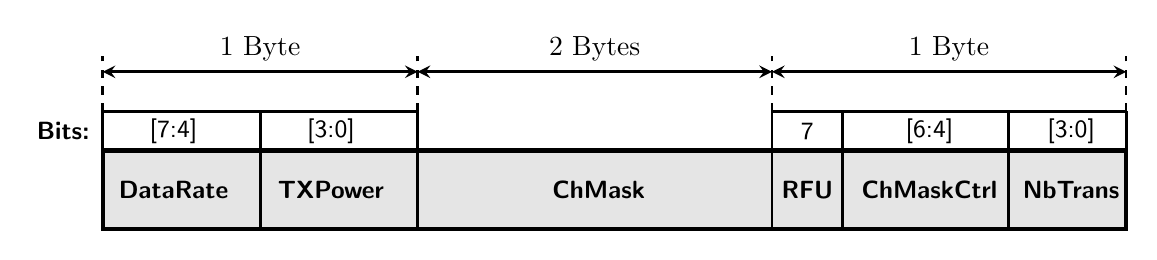
\begin{tikzpicture}
				\tikzset{
					defaulttext/.style={
						font=\sffamily\small,
					},
					smallText/.style={
						font=\sffamily\footnotesize,
					},
					defaultDashed/.style={dashed,line width=0.03cm},
					lineDef/.style={line width={1.5pt}},
					lineScaled/.style={line width={1pt}},
					arrowStyle/.style={lineScaled, >=stealth},
				}
				\draw[lineDef, fill=gray!20] (0,0) rectangle (13, 1.0);
				
				\foreach \x in {0, 2, 4, 8.5, 9.4, 11.5, 13} {
					\draw[lineScaled] (\x, 0) -- (\x, 1.5);
				}
				\foreach \x in {0, 4, 8.5, 13} {
					\draw[defaultDashed] (\x, 1.5) -- (\x, 2.2);
				}
				
				\draw[lineDef] (0,1) -- (13, 1);
				\draw[lineScaled] (0,1.5) -- (4, 1.5);
				\draw[lineScaled] (8.5,1.5) -- (13, 1.5);
				
				\node[defaulttext] at (0.9, 0.5) {\textbf{DataRate}};
				\node[defaulttext] at (0.9, 1.25) {\text{[7:4]}};
				\node[defaulttext] at (2.9, 0.5) {\textbf{TXPower}};
				\node[defaulttext] at (2.9, 1.25) {\text{[3:0]}};
				\node[defaulttext] at (6.3, 0.5) {\textbf{ChMask}};
				\node[defaulttext] at (8.95, 0.5) {\textbf{RFU}};
				\node[defaulttext] at (8.95, 1.25) {\text{7}};
				\node[defaulttext] at (10.5, 0.5) {\textbf{ChMaskCtrl}};
				\node[defaulttext] at (10.5, 1.25) {\text{[6:4]}};
				\node[defaulttext] at (12.3, 0.5) {\textbf{NbTrans}};
				\node[defaulttext] at (12.3, 1.25) {\text{[3:0]}};
				\node[defaulttext] at (-0.5, 1.25) {\textbf{Bits:}};
				
				%size
				\draw[arrowStyle, <->] (0, 2) -- node[midway, above] {1 Byte} (4,2);
				\draw[arrowStyle, <->] (4, 2) -- node[midway, above] {2 Bytes} (8.5,2);
				\draw[arrowStyle, <->] (8.5, 2) -- node[midway, above] {1 Byte} (13,2);
				
			\end{tikzpicture}
			\caption{Struktur des \PYTHON{LinkADRReq} Paket \cite{LoRaAlliance:2020b}}
		\end{figure}
		
		
		\begin{figure}[H]
			\centering
			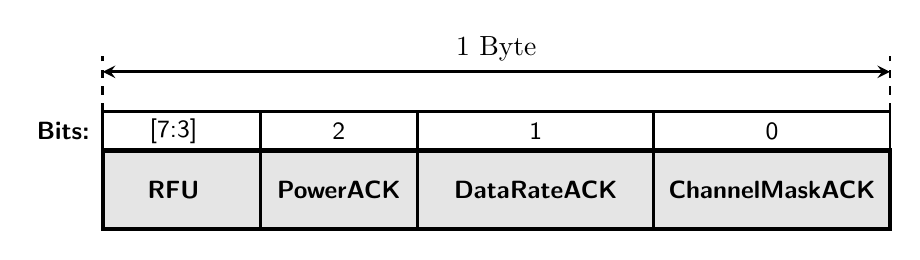
\begin{tikzpicture}
				\tikzset{
					defaulttext/.style={
						font=\sffamily\small,
					},
					smallText/.style={
						font=\sffamily\footnotesize,
					},
					defaultDashed/.style={dashed,line width=0.03cm},
					lineDef/.style={line width={1.5pt}},
					lineScaled/.style={line width={1pt}},
					arrowStyle/.style={lineScaled, >=stealth},
				}
				\draw[lineDef, fill=gray!20] (0,0) rectangle (10, 1.0);
				
				\foreach \x in {0, 2, 4, 7 ,10} {
					\draw[lineScaled] (\x, 0) -- (\x, 1.5);
				}
				
				\foreach \x in {0, 10} {
					\draw[defaultDashed] (\x, 1.5) -- (\x, 2.2);
				}
				
				\draw[lineScaled] (0,1.5) -- (10, 1.5);
				
				\node[defaulttext] at (0.9, 0.5) {\textbf{RFU}};
				\node[defaulttext] at (0.9, 1.25) {\text{[7:3]}};
				\node[defaulttext] at (3, 0.5) {\textbf{PowerACK}};
				\node[defaulttext] at (3, 1.25) {\text{2}};
				\node[defaulttext] at (5.5, 0.5) {\textbf{DataRateACK}};
				\node[defaulttext] at (5.5, 1.25) {\text{1}};
				\node[defaulttext] at (8.5, 0.5) {\textbf{ChannelMaskACK}};
				\node[defaulttext] at (8.5, 1.25) {\text{0}};
				\node[defaulttext] at (-0.5, 1.25) {\textbf{Bits:}};
				
				%size
				\draw[arrowStyle, <->] (0, 2) -- node[midway, above] {1 Byte} (10,2);
				
			\end{tikzpicture}
			\caption{Struktur des \PYTHON{LinkADRAns} Paket \cite{LoRaAlliance:2020b}}
		\end{figure}
	\end{itemize}
	
	\vspace{0.5cm}
	Diese MAC-Kommandos werden entweder im \PYTHON{FOpts}-Feld oder im \PYTHON{FRMPayload} übertragen, 
	wenn \PYTHON{FPort} = 0 ist \cite{LoRaAlliance:2020b}.
	
\subsection{Frame Counter (\PYTHON{FCnt})}
	LoRaWAN verwendet für jedes Endgerät zwei getrennte Zähler: den \PYTHON{FCntUp} für Uplink-Rahmen und den \PYTHON{FCntDown} für Downlink-Rahmen. Das Endgerät erhöht \PYTHON{FCntUp} bei jeder neu übertragenen Uplink-Nachricht, während der \ac{lns} den Wert \PYTHON{FCntDown} bei jedem an das Endgerät gerichteten Downlink fortschreibt. Beide Kommunikationspartner verwalten somit jeweils einen lokalen Zähler für die von ihnen gesendeten Rahmen sowie einen synchronisierten Zähler für empfangene Rahmen des Gegenübers.

	Bei einem erfolgreichen \ac{otaa}-Join werden beide Zähler auf~0 zurückgesetzt. Bei \ac{abp}-Endgeräten erfolgt die Initialisierung einmalig durch den Hersteller und darf während der gesamten Lebensdauer des Geräts nicht erneut durchgeführt werden. Endgeräte, die anfällig für Stromunterbrechungen sind (beispielsweise durch Batteriewechsel), müssen die aktuellen Zählerstände dauerhaft speichern.

	Nach der Aktivierung wird der aktuelle Zählerstand in jeder gesendeten Nachricht im Feld \PYTHON{FCnt} eingetragen: Uplink-Rahmen enthalten ausschlie{\ss}lich den Wert \PYTHON{FCntUp}, während Downlink-Rahmen den vom \ac{lns} vergebenen \PYTHON{FCntDown}-Wert enthalten. Beide Zähler sind intern 32~Bit breit; das im Rahmen übertragene Feld \PYTHON{FCnt} umfasst jedoch nur die niederwertigen 16~Bit des entsprechenden 32-Bit-Zählers.

	Auf Empfängerseite wird ein Rahmen nur dann akzeptiert, wenn der empfangene Zählerwert grö{\ss}er ist als der lokal gespeicherte Wert und der \PYTHON{MIC} korrekt verifiziert werden kann. Liegt der empfangene Zählerstand unterhalb des erwarteten Werts oder entspricht er einem bereits verarbeiteten Rahmen, wird die Nachricht verworfen. Dieses Verhalten schützt wirksam vor Replay-Angriffen und verhindert eine doppelte Verarbeitung derselben Nachricht \cite{Montagny:2022}.

	Wiederholte Übertragungen derselben Uplink-Nachricht (Retransmissions), die durch den Parameter \PYTHON{NbTrans} gesteuert werden (siehe~\autoref{lorawan:nbTrans}), erhöhen den \PYTHON{FCntUp}-Wert nicht. Der \ac{lns} muss dabei mögliche Duplikate erkennen und sicherstellen, dass die Nutzlast nur einmal an den Anwendungserver weitergereicht wird. Ebenso dürfen wiederholte Downlink-Rahmen mit identischem \PYTHON{FCntDown}-Wert vom Endgerät nicht erneut verarbeitet werden \cite{LoRaAlliance:2020b}.

\section{Kanäle}
	\ac{lora} nutzt in Europa das Frequenzband bei 868\,MHz (863\,MHz bis 870\,MHz). Innerhalb dieses Bandes definiert das \ac{lns} die verwendeten Kanäle und Datenraten für Uplink- und Downlink-Übertragungen. Unabhängig von der Netzwerkkonfiguration müssen jedoch alle \ac{lorawan}-Endgeräte drei LoRa-Modulationskanäle obligatorisch unterstützen:

	\begin{table}[H]
		\centering
		\begin{tabular}{|c|c|c|c|c|}
			\hline
			\textbf{{Bandbreite}} & 
			\textbf{{Kanalfrequenz}} & 
			\textbf{{LoRa Datenrate}} &
			\textbf{Duty-Cycle} \\
			
			\textbf{[kHz]} & 
			\textbf{[MHz]} & 
			\textbf{und Bitrate} & \\ 
			\hline
			125 & 868.10 & \shortstack{DR0 bis DR5 \\ 0.3 - 5 kbps} & <1\% \\
			\hline
			125 & 868.30 & \shortstack{DR0 bis DR5 \\ 0.3 - 5 kbps} & <1\% \\
			\hline
			125 & 868.50 & \shortstack{DR0 bis DR5 \\ 0.3 - 5 kbps} & <1\% \\
			\hline
		\end{tabular}
		\caption{Standardkanäle für das EU863--870-Frequenzband \cite{LoRaAlliance:2022}}
	\end{table}

	Diese drei Standardkanäle bilden die Grundlage jeder LoRaWAN-Kommunikation im EU-Band; insbesondere werden alle \textbf{Join-Requests} über diese Kanäle übertragen \cite{LoRaAlliance:2022}. Zusätzlich zu diesen Pflichtkanälen definiert \textcite{ETSI:2018} weitere zulässige Frequenzen im EU863--870-Band:

	\begin{table}[H]
		\centering
		\begin{tabular}{|c|c|c|c|}
			\hline
			\textbf{Kanal} & \textbf{Frequenz [MHz]} & \textbf{Duty Cycle} & \textbf{Richtung} \\
			\hline
			1 & 867.10  & 1\%  & Uplink / Downlink \\
			\hline
			2 & 867.30  & 1\%  & Uplink / Downlink \\
			\hline
			3 & 867.50  & 1\%  & Uplink / Downlink \\
			\hline
			4 & 867.70  & 1\%  & Uplink / Downlink \\
			\hline
			5 & 867.90  & 1\%  & Uplink / Downlink \\
			\hline
			9 & 869.525 & 10\% & Downlink only \\
			\hline
		\end{tabular}
		\caption{EU863--870 Kanäle mit Bandbreite 125\,kHz \cite[Kap.~7.2.1]{ETSI:2018}}
		\label{tab:eu868channels125}
	\end{table}

	Diese Kanäle sind nicht frei wählbar, sondern stammen aus den durch \textcite{ETSI:2018} sowie die Regionalparameter der \textcite{LoRaAlliance:2022} definierten Subbändern. Ein \ac{lns} darf somit ausschlie{\ss}lich Kanäle aktivieren, die innerhalb dieser regulierten Frequenzbereiche liegen. Endgeräte können nur solche Frequenzen nutzen, die sowohl regulatorisch zulässig als auch vom Netzwerkserver über MAC-Kommandos (\PYTHON{NewChannelReq}, \PYTHON{LinkADRReq}) freigegeben wurden \cite{LoRaAlliance:2020b, LoRaAlliance:2022}.


	Darüber hinaus definiert LoRaWAN eine \textit{Fixed Channel List} mit insgesamt 40 möglichen Frequenzen, die über die \PYTHON{CFList} im Join-Accept aktiviert werden können. \PYTHON{Channel-ID 0} entspricht 863{,}1\,MHz; jede weitere ID erhöht die Frequenz um 200\,kHz. Die IDs 35--39 repräsentieren fünf zusätzliche Frequenzen im Bereich 865{,}0625 - 865{,}985\,MHz. Für jedes in der \PYTHON{CFList} gesetzte Bit erstellt das Endgerät einen weiteren Kanal. Die Nummerierung dieser zusätzlichen Kanäle beginnt stets hinter den drei Standardkanälen, also bei \PYTHON{ChIndex} = 3, wodurch eine eindeutige und konsistente Kanalstruktur zwischen Endgerät und Netzwerkserver gewährleistet wird \cite[30 - 31]{LoRaAlliance:2022} \cite[36]{LoRaAlliance:2020b}.


	Beim \PYTHON{Over-the-Air Activation} (OTAA) kann der Netzwerkserver während des Join-Prozesses zusätzliche Kanäle und Datenraten an das Endgerät übermitteln – entweder über die \PYTHON{CFList} im Join-Accept oder über spätere MAC-Kommandos. Bei der \ac{abp} hingegen erhält das Endgerät keine dynamischen Kanalparameter vom Netzwerkserver. In diesem Fall nutzt es ausschlie{\ss}lich die drei Pflichtkanäle, sofern zusätzliche Kanäle nicht manuell im Firmware-Design hinterlegt wurden \cite{LoRaAlliance:2022, Montagny:2022}.


\subsection{Datenrate (\PYTHON{DR}) \label{lorawan:dataRate}}
	Die LoRaWAN-Datenrate (\PYTHON{DR}) definiert einen fest vorgegebenen Übertragungsmodus, der aus einer Kombination von Spreading Factor (SF), Bandbreite (BW) besteht. Jede \PYTHON{DR} entspricht somit einem vollständigen Profil, dessen physikalische Bitrate direkt aus diesen Parametern hervorgeht. Höhere SF-Werte führen zu einer geringeren Bitrate, ermöglichen jedoch grö{\ss}ere Reichweiten; niedrigere SF-Werte bieten höhere Datenraten bei kürzerer Reichweite. Die Zuordnung der standardisierten Datenraten ist in der \textcite{LoRaAlliance:2022} spezifiziert und in \autoref{tab:datarate} dargestellt.

	\begin{table}[H]
		\centering
		\begin{tabular}{|c|c|c|}
			\hline
			\textbf{Data Rate} & \textbf{Konfiguration} & \textbf{Physikalische Bitrate [bit/s]}\\
			\hline
			0 &SF12 / 125 kHz & 250 \\
			\hline
			1 & SF11 / 125 kHz & 440 \\
			\hline
			2 & SF10 / 125 kHz & 980 \\
			\hline
			3 & SF9 / 125 kHz & 1760 \\
			\hline
			4 & SF8 / 125 kHz & 3125 \\
			\hline
			5 & SF7 / 125 kHz & 5470 \\
			\hline
			6 & SF7 / 250 kHz & 11000 \\
			\hline
		\end{tabular}
		\caption{Datenraten im EU863 - 870-Frequenzband}
		\label{tab:datarate}
	\end{table}


\section{Duty Cycle}
	Hier gelten dieselben Vorschriften, die auch bei LoRa zur Anwendung kommen. Das europäische ISM-Band ist gemä{\ss} \citeauthor[22]{ETSI:2018b} in mehrere Sub-Bänder unterteilt, von denen sechs (K, L, M, N, P, Q) für LoRa- und LoRaWAN-Anwendungen relevant sind. Jedes dieser Sub-Bänder besitzt spezifische Beschränkungen hinsichtlich des zulässigen Duty Cycle sowie der maximalen äquivalenten Strahlungsleistung (ERP). Diese Vorgaben beeinflussen unmittelbar, welche Kanäle genutzt werden dürfen und wie häufig ein Gerät innerhalb der jeweiligen Frequenzbereiche senden kann.
	
	
	\begin{table}[H]
		\centering
		\begin{tabular}{|c|c|c|c|}
			\hline
			\textbf{Sub-Band} & \textbf{Frequenzbereich [MHz]} & \textbf{Duty Cycle} & \textbf{Max. ERP} \\
			\hline
			K & 863.0--865.0   & 0.1\,\%  & 25\,mW \\
			\hline
			L & 865.0--868.0   & 1\,\%    & 25\,mW \\
			\hline
			M & 868.0--868.6   & 1\,\%    & 25\,mW \\
			\hline
			N & 868.7--869.2   & 0.1\,\%  & 25\,mW \\
			\hline
			P & 869.4--869.65  & 10\,\%   & 500\,mW \\
			\hline
			Q & 869.7--870.0   & 1\,\%    & 25\,mW \\
			\hline
		\end{tabular}
		\caption{ETSI-Unterbänder im EU863--870-Band mit Duty-Cycle-Restriktionen 
			\cite{ETSI:2018b}}
	\end{table}
	
\section{Energieverbrauch}
	Der Energieverbrauch eines LoRaWAN-Endgeräts wird im Wesentlichen durch die physikalischen Eigenschaften der LoRa-Modulation sowie die in LoRaWAN definierten Empfangs- und Sendeprozesse bestimmt. Da viele LoRaWAN-Geräte batteriebetrieben sind, spielt die Minimierung des Energiebedarfs eine zentrale Rolle bei der Auslegung von Applikationen und der Wahl geeigneter Betriebsparameter \cite{Montagny:2022}.

	Gro{\ss}e Energieanteil entsteht während der Funkübertragung. Die Dauer einer Übertragung hängt direkt vom gewählten Spreading Factor (SF), der Bandbreite (BW), der Sendeleistung und der Payload-Grö{\ss}e ab. Höhere SF-Werte vergrö{\ss}ern die Airtime eines Frames und erhöhen den Energieverbrauch signifikant, ermöglichen jedoch grö{\ss}ere Reichweiten. Eine typische Übertragung mit SF12 benötigt ein Vielfaches der Zeit und Energie im Vergleich zu einem Senden mit SF7 \cite{ETSI:2018} \cite{Montagny:2022}.

	Neben der eigentlichen Sendephase tragen auch die durch LoRaWAN definierten Empfangsfenster zum Energieverbrauch bei. Bei Geräten der Klasse~A müssen nach jedem Uplink zwingend zwei Empfangsfenster (RX1 und RX2) geöffnet werden, unabhängig davon, ob ein Downlink erwartet wird. Bei Geräten der Klasse~C wird das Fenster RXC die ganze Zeit geöffnet. Diese Aktivitätsphasen im Empfangsmodus stellen einen bedeutenden Faktor im Gesamtenergieverbrauch dar \cite{LoRaAlliance:2020b}.

	Der zusätzliche Energieaufwand steigt bei der Verwendung bestätigter Nachrichten (\textit{Confirmed Frames}), da ein fehlendes \PYTHON{ACK} zur erneuten Übertragung desselben Frames führt. Auch die Anzahl der Wiederholungen (\PYTHON{NbTrans}) und die durch ADR gewählten Parameter (insbesondere die Datenrate) beeinflussen direkt die Leistungsaufnahme. Ein effizient konfigurierter ADR-Mechanismus kann den Energieverbrauch deutlich senken, indem er die Datenrate und Sendeleistung an die aktuellen Funkbedingungen anpasst \cite{LoRaAlliance:2020b}.

	Um einen möglichst niedrigen Energieverbrauch zu erreichen, werden LoRaWAN-Geräte zwischen den Übertragungen in stromsparende Schlafmodi versetzt \cite{Semtech:2024}. Die gesamte Energieeffizienz hängt daher stark von der Anwendung ab: Geräte, die selten senden und mit niedrigen SF-Werten arbeiten, erreichen üblicherweise Batterielaufzeiten von mehreren Jahren, während häufige Übertragungen oder hohe SF-Werte den Energiebedarf entsprechend steigern.



%\section{Anwendungsbeispiele}
%LoRaWAN wird in städtischen Sensornetzwerken, intelligenten Zählern, Logistiksystemen oder Agrarprojekten eingesetzt.
%\section{Bibliothek}
%\section{Beispielcode}
